\section{Complexity}

  Therefore, if we apply it to some binary classifier $f: \mathcal{X} \rightarrow \{0, 1\}$, then we can say that the probability that the empirical risk deviates from the true risk is exponentially small. 
  \begin{equation}
    \mathbb{P} (|\hat{R} (f) - R(f)| \geq \epsilon) \leq 2e^{- 2 n \epsilon^2}
  \end{equation}
  But when we do empirical risk minimization (ERM), we not given a classifier, but we must \textit{choose} it. So given our space of classifiers $f$, we can plot the true risk and the noisy empirical risk. The equation above states that at any given point the probability of it deviating by more than $\epsilon$ is exponentially small. But we want something stronger: we want to bound the probability of the supremum of the difference over the whole class $\mathcal{F}$. 

  \begin{figure}[H]
    \centering 
    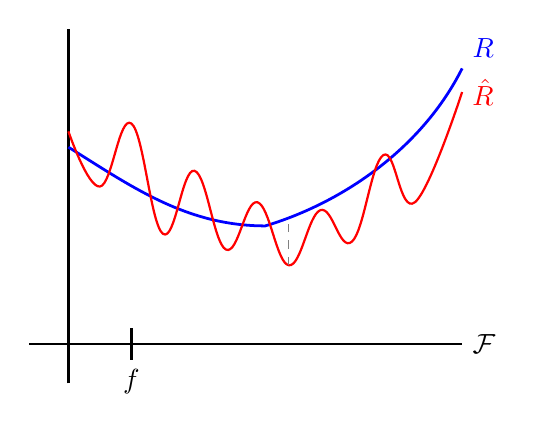
\begin{tikzpicture}
      \draw[black, line width=1pt] (-0.5,0) -- (5,0) node[right] {$\mathcal{F}$};
      \draw[black, line width=1pt] (0,-0.5) -- (0,4);

      \draw[black, line width=0.8pt] (0.8,-0.2) -- (0.8,0.2);
      \node[below] at (0.8,-0.2) {$f$};
      
      \draw[blue, line width=1pt] 
        (0,2.5) .. controls (0.8,2) and (1.5,1.5) .. 
        (2.5,1.5) .. controls (3.5,1.8) and (4.5,2.5) .. 
        (5,3.5) node[above right] {$R$};
        
      \draw[red, line width=0.8pt]
        plot[smooth, tension=0.7] coordinates {
          (0,2.7) (0.4,2.0) (0.8,2.8) (1.2,1.4) (1.6,2.2)
          (2.0,1.2) (2.4,1.8) (2.8,1.0) (3.2,1.7) (3.6,1.3)
          (4.0,2.4) (4.4,1.8) (5,3.2)
        } node[right] {$\hat{R}$};

      \draw[gray, dashed] (2.8,1.0) -- (2.8,1.6);
    \end{tikzpicture}
    \caption{True risk of functions over $\mathcal{F}$ and its noisy empirical risk. We want to bound the maximum deviation of these two over the whole class.} 
    \label{fig:true_vs_empirical_risk}
  \end{figure}

  By taking the supremum, this bound comes at a cost in the form of a coefficient term $C$. 
  \begin{equation}
    \mathbb{P} \big( \sup_{f \in \mathcal{F}} | \hat{R} (f) - R(f) | \geq \epsilon \big) \leq C e^{-2 n \epsilon^2}
  \end{equation}

  This constant $C$---and the bound---will depend on how \textit{complex} the function class $\mathcal{F}$ is, and to measure this complexity, we introduce some definitions. 

\subsection{Rademacher Complexity}

  \begin{definition}[Rademacher Complexity]
    Given \textbf{Rademacher random variables} $\sigma_1, \ldots, \sigma_n$ with $\mathbb{P}(\sigma_i = 1) = \mathbb{P}(\sigma_i = -1) = \frac{1}{2}$, the \textbf{Rademacher complexity} of a function class $\mathcal{F}$ is defined 
    \begin{equation}
      \mathrm{Rad}_n (\mathcal{F}) = \mathbb{E} \bigg[ \sup_{f \in \mathcal{F}} \bigg| \frac{1}{n} \sum_{i=1}^n \sigma_i f(Z_i) \bigg| \bigg]
    \end{equation}
    where the expectation is across the random $\sigma_i$'s and the $Z_i$'s, which are independent. 
  \end{definition}

  To get some intuition of what this is, let's consider a function class of a single function $f$. Then, the sup disappears and the term inside the absolute value sign becomes a $0$-mean random variable. Now if we have a very complex function class $\mathcal{F}$ with a lot of ``wiggly'' functions, then this value should be large. In this case, imagine a game where you pick generate some random variables $\sigma_i$ and the $Z_i$. Then, I pick a function that maximizes this value. How can I do that? If I can find a function $f$ that matches the sign of the $\sigma_i$'s ($+1$ or $-1$) at each of the values of $Z_i$, then this would be maximized. 

  \begin{figure}[H]
    \centering
    \begin{subfigure}[b]{0.48\textwidth}
      \centering
      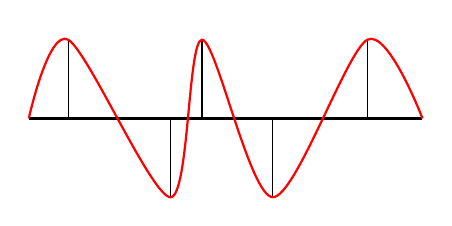
\begin{tikzpicture}
        % Draw horizontal line
        \draw[thick] (1,0) -- (6,0);

        % Draw 5 vertical lines at specific positions
        \draw (1.5,0) -- (1.5,1);
        \draw (2.8,0) -- (2.8,-1);
        \draw (3.2,0) -- (3.2,1);
        \draw (4.1,0) -- (4.1,-1);
        \draw (5.3,0) -- (5.3,1);

        % Draw smooth curve through points in x-order
        \draw[red, thick] plot[smooth] coordinates {
         (1,0) (1.5,1) (2.8,-1) (3.2,1) (4.1,-1) (5.3,1) (6,0)
        };
      \end{tikzpicture}
      \caption{One round of the game. }
    \end{subfigure}
    \hfill 
    \begin{subfigure}[b]{0.48\textwidth}
      \centering
      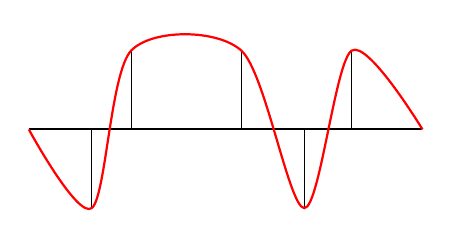
\begin{tikzpicture}
        % Draw horizontal line
        \draw[thick] (1,0) -- (6,0);

        % Draw 5 vertical lines at specific positions
        \draw (1.8,0) -- (1.8,-1);
        \draw (2.3,0) -- (2.3,1);
        \draw (3.7,0) -- (3.7,1);
        \draw (4.5,0) -- (4.5,-1);
        \draw (5.1,0) -- (5.1,1);

        % Draw smooth curve through points in x-order
        \draw[red, thick] plot[smooth] coordinates {
         (1,0) (1.8,-1) (2.3,1) (3.7,1) (4.5,-1) (5.1,1) (6,0)
        };
      \end{tikzpicture}
      \caption{Another round of the game. }
    \end{subfigure}
    \caption{Given the 5 random points $Z_i$ chosen on the horizontal axis and their directions given by $\sigma_i$, we would like to find a function $f \in \mathcal{F}$ that interpolates the points.}
    \label{fig:game}
  \end{figure}

  Therefore, if I have a sufficiently complex class, then I can pick a function that tracks your $\sigma_i$'s. Another way of looking at it is given noise variables $\sigma$ and $Z$, we're looking at the correlation between $\sigma$ and $f(Z)$. If we can maximize this correlation, then this is a complex class. 

  This is the most natural way of defining the complexity of the class, and in some cases it can be explicitly computed. However, in most cases it cannot be, but it can be bounded be something that is computable, like the VC dimension. 

  \begin{lemma}[Bigger Class, Bigger Complexity]
    If $\mathcal{F} \subset \mathcal{G}$, then $\mathrm{Rad}_n (\mathcal{F}) \leq \mathrm{Rad}_n (\mathcal{G})$.
  \end{lemma}

  \begin{lemma}[Convex Hull]
    If $\mathcal{F}$ is a convex set, then $\mathrm{Rad}_n (\mathcal{F}) = \mathrm{Rad}_n (\mathrm{conv}(\mathcal{F}))$, where $\mathrm{conv}(\mathcal{F})$ is the convex hull of $\mathcal{F}$.
  \end{lemma}

  This lemma is quite useful since if we have a certain finite set of functions, then their convex hull can encompass quite a bit, and we can also easily compute that convex hull's Rademacher complexity. Since the extremes haven't changed, the complexity doesn't change, and this might suggest that the Rademacher complexity is a good measure. 

  \begin{lemma}[Change of Complexity with Lipschitz Functions]
    Consider a $L$-Lipschitz function $g$  with $g(0) = 0$ and consider the class $\mathcal{F}$, then we can bound the class of functions $g \circ \mathcal{F} = \{ g \circ f \mid f \in \mathcal{F} \}$. 
    \begin{equation}
      \mathrm{Rad}_n (g \circ \mathcal{F}) \leq 2 L \mathrm{Rad}_n (\mathcal{F})
    \end{equation}
    This constant multiplicative bound is also useful. 
  \end{lemma}

\subsection{Shattering Numbers}

  \begin{definition}[Projection of Function Class onto Points]
    Given a binary function class $\mathcal{F}$ with functions $f: \mathcal{X} \rightarrow \{0, 1\}$, let us denote the projection of $\mathcal{F}$ onto a set of points $z_1, \ldots, z_n \in \mathcal{X}$ to be 
    \begin{equation}
      \mathcal{F}_z = \mathcal{F}_{z_1, \ldots, z_n} = \{ (f(z_1), \ldots, f(z_n)) \mid f \in \mathcal{F} \} \subset \{0, 1\}^n
    \end{equation}
  \end{definition}

  This projection determines the set of all possible binary labels that can be perfectly classified by some function $f$. 

  \begin{definition}[Shattering Number]
    The \textbf{shattering number} of $\mathcal{F}$ is defined 
    \begin{equation}
      s_n (\mathcal{F}) = s(\mathcal{F}, n) = \sup_{z_1, \ldots, z_n} |\mathcal{F}_{z_1, \ldots, z_n}|
    \end{equation}
    In other words, given the points $z_j$, how many different labels (out of the $2^n$ possible ones) can we put on the $z_j$ so that there exists a function $f \in \mathcal{F}$ that can perfectly classify the $z_j$'s? For every set of points you'll get a different integer. Now take the supremum. 
  \end{definition}

  The highest number that this can be is $2^n$, since this is the number of possible binary vectors of length $n$. 

  \begin{definition}[Shattering a Set]
    Given a set of $n$ points $z_1, \ldots, z_n$, we say that the function class $\mathcal{F}$ \textbf{shatters} this set if $\mathcal{F}_{z_1, \ldots, z_n} = |2^n|$. That is, for \textit{every} one of the $2^n$ labels on these points, there exists a function in $\mathcal{F}$ that can perfectly classify them. 
  \end{definition}

  Therefore, if $\mathcal{F}$ shatters a set, the function class is in a sense too powerful to use on the dataset, since no matter what labels we put on the data, there exists a perfect function that interpolates it. 

  \begin{example}[Binary Functions]
    Consider the function class $\mathcal{F}$ of all binary functions of the form 
    \begin{equation}
      f(x) = \begin{cases} 1 & \text{ if } x > t \\
        0 & \text{ if } x \leq t \end{cases} 
    \end{equation}
    Then, the projection of $\mathcal{F}$ onto some $n = 3$ points is the set 
    \begin{equation}
      \{ (0, 0, 0), (0, 0, 1), (0, 1, 1), (1, 1, 1) \}
    \end{equation}
    and this is true no matter how I pick the $z_1, z_2, z_3$, and so the Shattering number is $s_3 (\mathcal{F}) = 4$. 
  \end{example}

  What is great about the shattering number is that it can be used to upper bound the Rademacher complexity. Often times, we do not know the Rademacher complexity but know the shattering number. 

  \begin{theorem}[Bound of Rademacher Complexity with Shattering Number]
    The Rademacher complexity of a binary function class $\mathcal{F}$ is bounded by 
    \begin{equation}
      \mathrm{Rad}_n (\mathcal{F}) \leq \sqrt{\frac{2 \log s_n (\mathcal{F})}{n}}
    \end{equation}
  \end{theorem}
  \begin{proof}
    Given the projection $\mathcal{F}_{z_1, \ldots, z_n}$, we can use the law of iterated expectations on the Rademacher complexity. 
    \begin{align}
      \mathrm{Rad}_n (\mathcal{F}) & = \mathbb{E}_{Z, \sigma} \bigg[ \sup_{f \in \mathcal{F}} \bigg| \frac{1}{n} \sum_{i=1}^n \sigma_i f(Z_i) \bigg| \bigg] \\
                                   & = \mathbb{E}_{Z} \bigg[ \mathbb{E}_{\sigma} \bigg[ \sup_{f \in \mathcal{F}} \bigg| \frac{1}{n} \sum_{i=1}^n \sigma_i f(Z_i) \bigg| \; \mid \; Z_1, \ldots Z_n \bigg] \bigg] 
    \end{align}
    Note that in the inner expectation, since $f(Z_i)$ is now fixed, then are bounding a linear combination of a bunch of $\sigma_i$'s. Note that since $f$ is binary, 
    \begin{equation}
      0 \leq f(Z_i) \leq 1 \implies -1 \leq \sigma_i f(Z_i)\leq 1 \implies -1 \leq \frac{1}{n} \sum_{i=1}^n \sigma_i f(Z_i) \leq 1 
    \end{equation}
    and so it is subgaussian, satisfying 
    \begin{equation}
      \mathbb{E}\left[ \exp \left( \lambda \frac{1}{n} \sum_{i=1}^n \sigma_i f(Z_i) \right)\right] \leq \exp \left( \frac{2 \lambda^2}{2} \right)
    \end{equation}
    where $\sigma = 2$. Using \ref{subgaussian_bound}, we can reduce it to 
    \begin{align}
      \mathbb{E}_{\sigma_i} \left[ \sup_{f \in \mathcal{F}} \left| \frac{1}{n} \sum_{i=1}^n \sigma_i f(Z_i) \right| \mid Z_1, \ldots, Z_n \right] 
      & = \mathbb{E}_{\sigma_i} \left[ \max_{f \in \mathcal{F}} \left| \frac{1}{n} \sum_{i=1}^n \sigma_i f(Z_i) \right| \mid Z_1, \ldots, Z_n \right] \\
      & = \mathbb{E}_{\sigma_i} \left[ \max_{\substack{(f(Z_1), \ldots, f(Z_n)) \\ \in \mathcal{F}_{z_1, \ldots, z_n}}} \left| \frac{1}{n} \sum_{i=1}^n \sigma_i f(Z_i) \right| \mid Z_1, \ldots, Z_n \right] \\
      & \leq 2 \sqrt{2 \log{| F_{z_1, \ldots, z_n}|}} \\
      & \leq 2 \sqrt{2 \log{s_n (\mathcal{F})}}
    \end{align}
    where in the penultimate step, we have used the fact that $Z_i$'s are fixed in order to prove that maximizing over $\mathcal{F}$ is the same as maximizing over the projection values. We can then unfix the $Z_i$'s, but at this point the random variable isn't even dependent on them, so the expectation reduces to 
    \begin{equation}
      \mathbb{E} \left[ 2 \sqrt{2 \log{s_n (\mathcal{F})}} \right] = 2 \sqrt{2 \log{s_n (\mathcal{F})}}
    \end{equation}
  \end{proof}

  However, this is not the best possible bound, and in cases such as K means clustering in high dimensions, this bound can be tightened. 

\subsection{VC Dimension}

  We know that the shattering number is bounded above by $2^n$. For $n = 1$, it is reasonable that it achieves this bound, but as $n$ grows, the Shattering number may die off. The point at which it dies off is precisely the VC dimension.  

  \begin{definition}[VC Dimension]
    The \textbf{VC dimension} is the largest $n$ number of points that can be shattered by the function class without misclassification \cite{1971vapnik}. 
    \begin{equation}
      n^{\mathrm{VC}} \coloneqq \sup_n \{ s_n (\mathcal{F}) = 2^n \}
    \end{equation}

    \begin{figure}[H]
      \centering 
      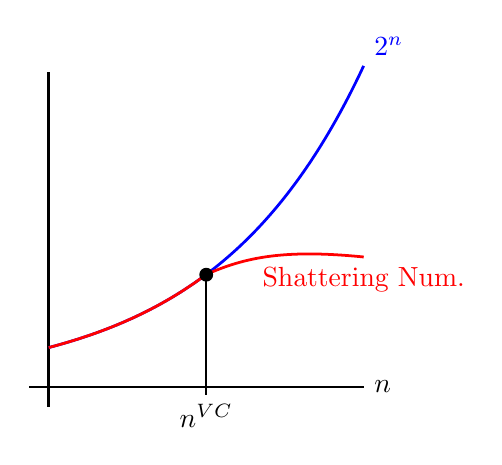
\begin{tikzpicture}[scale=0.5]
        % Draw axes
        \draw[black, line width=1pt] (-0.5,0) -- (8,0) node[right] {$n$};
        \draw[black, line width=1pt] (0,-0.5) -- (0,8);
        
        % Draw 1.1^x curve (blue)
        \draw[blue, line width=1pt] 
          plot[domain=0:8, smooth, samples=100] 
          (\x, {1.3^\x}) node[above right] {$2^n$};
          
        % Draw Shattering Number curve (red) - matches 1.1^x until VC Dim
        \draw[red, line width=1pt]
          plot[domain=0:4, smooth, samples=50] (\x, {1.3^\x})
          .. controls (5,3.3) and (6,3.5) ..
          (8,3.3) node[below] {Shattering Num.};
          
        % Mark VC Dimension / Shattering Number
        \draw[black, line width=0.8pt] (4,-0.2) -- (4,2.85);
        \node[below] at (4,-0.2) {$n^{VC}$};
        
        % Mark intersection point
        \fill[black] (4,2.85) circle (5pt);
      \end{tikzpicture}
      \caption{The Shattering number of $\mathcal{F}$ will grow exponentially until it reaches the VC dimension, at which point it will grow polynomially. The point at which it ``dies off'' is the VC dimension.} 
      \label{fig:sawyer_lemma}
    \end{figure}
  \end{definition}

  It turns out that there are very interesting properties about the VC dimension. One such fact is Sauer's lemma, which states that if the VC dimension is finite, then the rate of growth of the shattering number suddenly changes from exponential $2^n$ to polynomial $n^{\mathrm{VC}}$, and this is what makes a lot of machine learning work. 

  \begin{lemma}[Sauer–Shelah Lemma]
    When the VC dimension $n^{VC}$ of a function class $\mathcal{F}$ is finite, then for $n > n^{VC}$, the shattering number is bounded as 
    \begin{equation}
      s_n (\mathcal{F}) \leq \left( \frac{\epsilon n}{d} \right)^d
    \end{equation}
    which grows polynomially in $n$. 
  \end{lemma}
  \begin{proof}
    
  \end{proof}

  Therefore, if we use this lemma on the shattering number bound on the Rademacher complexity, we get 
  \begin{equation}
    \mathrm{Rad}_n (\mathcal{F}) \leq \sqrt{\frac{2 \log s_n (\mathcal{F})}{n}} \leq \sqrt{\frac{2 d \log{n}}{n}} 
  \end{equation}
  It turns out that with much longer proofs, the $\log{n}$ can be removed. 

  There are other types of complexity besides Rademacher that we will use when the VC dimension is infinite. 

  To prove this, we need a few tricks, the first being the symmetrization trick using ghost samples. 

  \begin{lemma}[Symmetrization Lemma]
    Given a set of random variables $Z_1, \ldots, Z_n$ and a function class $\mathcal{F}$, we can define ghost samples $Z_1^\prime, \ldots, Z_n^\prime$ that are iid copies of $Z_1, \ldots, Z_n$. Then, we can bound the Rademacher complexity of the function class $\mathcal{F}$ by 
    \begin{equation}
      \mathbb{P} \bigg( \sup_{f \in \mathcal{F}} | \hat{R} (f) - R(f) | \geq \epsilon \bigg) \leq 2 \mathbb{P} \bigg( \sup_{f \in \mathcal{F}} | \hat{R} (f) - \hat{R}^\prime (f) | \geq \epsilon / 2 \bigg)
    \end{equation}
    where $\hat{R}, \hat{R}^\prime$ is the empirical risk over the original and ghost samples, respectively. 
  \end{lemma}
  \begin{proof}
    Assume that we have a function $f$ that achieves this minimum. By the triangle inequality, 
    \begin{equation}
      | \hat{R} (f) - R(f)| > t \text{ and } | \hat{R}^\prime (f) - R(f)| < \frac{t}{2} \implies | \hat{R} (f) - \hat{R}^\prime (f) | > \frac{t}{2}
    \end{equation}
    We write this again as an indicator function. 
    \begin{equation}
      \mathbbm{1} (| \hat{R} (f) - R(f)| > t, | \hat{R}^\prime (f) - R(f)| < \frac{t}{2}) \implies \mathbbm{1} (| \hat{R} (f) - \hat{R}^\prime (f) | > \frac{t}{2})
    \end{equation}
    and since the samples and the ghost samples are independent, we can take the probability over the ghost samples to get 
    \begin{equation}
      \mathbbm{1} (| \hat{R} (f) - R(f)| > t) \, \mathbb{P}_{Z^\prime} (| \hat{R}^\prime (f) - R(f)| < \frac{t}{2}) \implies \mathbb{P}_{Z^\prime} (| \hat{R} (f) - \hat{R}^\prime (f) | > \frac{t}{2})
    \end{equation}
    and the rest of the proof can be found online. 
  \end{proof}

  The reason we want this is that it removes the $R(f)$, which is some unknown true mean that can be hard to deal with since it takes infinite values. It's easier to work with two empirical risks than deal with the true risk. 

  Now we move onto the big VC theorem which now bounds the supremum of the difference between the empirical risk and the true risk. You can think of it as an extension to Hoeffding's inequality to \textit{classes} of functions. 

  \begin{theorem}[VC Theorem]
    Given a binary function class $\mathcal{F}$, we have
    \begin{equation}
      \mathbb{P} \bigg( \sup_{f \in \mathcal{F}} | \hat{R} (f) - R(f) | \geq \epsilon \bigg) \leq 2 S(\mathcal{F}, n) e^{-n \epsilon^2 / 8} \approx n^d e^{-n \epsilon^2 / 8}
    \end{equation}
    You can see that the exponential term is from Hoeffding but there is an extra cost of taking the supremum over the whole function class, which is the shattering number. Fortunately, with Sauer's lemma, we can see that the coefficient grows polynoimally but the rest decays exponentially. 
  \end{theorem}
  \begin{proof}
    Given $Z_1, \ldots, Z_n \sim \mathbb{P}$, we take a new set of random variables $Z_1^{\prime}, \ldots, Z_n^{\prime}$ that are iid copies of $Z_1, \ldots, Z_n$, called \textit{ghost samples}.
   
    We begin by relating the original probability to one involving ghost samples:
    \begin{align}
      \mathbb{P} \left( \sup_{f \in \mathcal{F}} | \hat{R}(f) - R(f) | \geq \epsilon \right) &= \mathbb{P} \left( \sup_{f \in \mathcal{F}} \left| \frac{1}{n} \sum_{i=1}^n f(Z_i) - \mathbb{E}[f(Z)] \right| \geq \epsilon \right)
    \end{align}
   
    Since $Z_1^{\prime}, \ldots, Z_n^{\prime}$ are independent copies of $Z$ with the same distribution, we have $\mathbb{E}[f(Z)] = \mathbb{E}\left[\frac{1}{n} \sum_{i=1}^n f(Z_i^{\prime})\right]$. Therefore:
    \begin{align}
      &= \mathbb{P} \left( \sup_{f \in \mathcal{F}} \left| \frac{1}{n} \sum_{i=1}^n f(Z_i) - \mathbb{E}\left[\frac{1}{n} \sum_{i=1}^n f(Z_i^{\prime})\right] \right| \geq \epsilon \right)
    \end{align}
   
    By Jensen's inequality and the convexity of the supremum:
    \begin{align}
      &\leq \mathbb{P} \left( \sup_{f \in \mathcal{F}} \left| \frac{1}{n} \sum_{i=1}^n f(Z_i) - \frac{1}{n} \sum_{i=1}^n f(Z_i^{\prime}) \right| \geq \epsilon \right)\\
      &= \mathbb{P} \left( \sup_{f \in \mathcal{F}} \left| \frac{1}{n} \sum_{i=1}^n (f(Z_i) - f(Z_i^{\prime})) \right| \geq \epsilon \right)
    \end{align}
   
    Introduce independent Rademacher random variables $\sigma_1, \ldots, \sigma_n$ (each taking values $\pm 1$ with probability $1/2$), independent of all $Z_i, Z_i^{\prime}$. Since $f(Z_i) - f(Z_i^{\prime})$ has a symmetric distribution around 0:
    \begin{align}
      &= \mathbb{P} \left( \sup_{f \in \mathcal{F}} \left| \frac{1}{n} \sum_{i=1}^n \sigma_i (f(Z_i) - f(Z_i^{\prime})) \right| \geq \epsilon \right)\\
      &\leq 2\mathbb{P} \left( \sup_{f \in \mathcal{F}} \frac{1}{n} \sum_{i=1}^n \sigma_i (f(Z_i) - f(Z_i^{\prime})) \geq \epsilon \right)
    \end{align}
   
    Conditioning on $Z_1, \ldots, Z_n, Z_1^{\prime}, \ldots, Z_n^{\prime}$, the supremum is taken over at most $S(\mathcal{F}, 2n)$ distinct functions on the combined sample $\{Z_1, \ldots, Z_n, Z_1^{\prime}, \ldots, Z_n^{\prime}\}$.
   
    For each fixed realization of the samples, we have at most $S(\mathcal{F}, 2n)$ different sign patterns, and for each pattern, $\sum_{i=1}^n \sigma_i (f(Z_i) - f(Z_i^{\prime}))$ is a sum of independent bounded random variables.
   
    For any fixed function $f$, since $f$ is binary-valued, $|f(Z_i) - f(Z_i^{\prime})| \leq 2$. By Hoeffding's inequality:
    \begin{align}
      \mathbb{P} \left( \frac{1}{n} \sum_{i=1}^n \sigma_i (f(Z_i) - f(Z_i^{\prime})) \geq \epsilon \right) \leq e^{-n\epsilon^2/8}
    \end{align}
   
    Taking the union bound over all possible functions in the restriction of $\mathcal{F}$ to the $2n$ samples:
    \begin{align}
      \mathbb{P} \left( \sup_{f \in \mathcal{F}} \frac{1}{n} \sum_{i=1}^n \sigma_i (f(Z_i) - f(Z_i^{\prime})) \geq \epsilon \right) &\leq S(\mathcal{F}, 2n) e^{-n\epsilon^2/8}
    \end{align}
   
    Since $S(\mathcal{F}, 2n) \leq S(\mathcal{F}, n)^2$ and using the fact that we're interested in the bound in terms of $S(\mathcal{F}, n)$:
    \begin{align}
      \mathbb{P} \left( \sup_{f \in \mathcal{F}} | \hat{R}(f) - R(f) | \geq \epsilon \right) &\leq 2 S(\mathcal{F}, n) e^{-n\epsilon^2/8}
    \end{align}
   
    By Sauer's lemma, if $\mathcal{F}$ has VC dimension $d$, then $S(\mathcal{F}, n) \leq \left(\frac{en}{d}\right)^d \approx n^d$ for large $n$, giving the final approximation.
  \end{proof}

  The key insight is that the ghost sample technique allows us to replace the unknown population risk with an empirical average over independent samples, enabling the application of concentration inequalities while paying the price of the shattering coefficient.

  Therefore, for some classes of sets with finite VC dimension, the shattering term will grow polynomially in $n$ but the exponential term decays faster, which is what makes this work. That's why as $n$ grows, we can get a good bound on the supremum of this difference. 

  \begin{theorem}
    We have 
    \begin{equation}
      \mathbb{P} \left( \sup_{f \in \mathcal{F}} |\hat{R} (f) - R(f)| \leq 2 \mathrm{Rad}_n (\mathcal{F}) + \sqrt{\frac{\log (2 / \delta)}{2 n}} \right) \geq 1 - \delta
    \end{equation}
  \end{theorem}

\subsection{Covering Numbers} 

  Given function class $\mathcal{F}$ with some metric $d$, we try to find a subset of functions $\mathcal{G} \subset \mathcal{F}$ such that 
  \begin{equation}
    \bigcup_{g \in G} B_\epsilon(g) = \mathcal{F}
  \end{equation}
  That is, the set of $\epsilon$-balls around each $g$ cover $\mathcal{F}$. 

\subsection{Bracketing Numbers} 

  
